% TMLR submission. Uses tmlr.sty when it is present next to this file.
\documentclass[10pt]{article}
\usepackage{tmlr}
\usepackage{hyperref}
\usepackage{url}
\usepackage{amsmath,amssymb,amsthm}
\usepackage{booktabs}
\usepackage{graphicx}
\usepackage{xcolor}
\usepackage{tikz}
\usetikzlibrary{arrows.meta,positioning,fit,calc}
\usepackage{enumitem}
\setlist{nosep,leftmargin=1.6em}
\newcommand{\pending}[1]{\textcolor{red}{[PENDING: #1]}}
\theoremstyle{definition}
\newtheorem{definition}{Definition}

\title{How Five Confound Detectors for Clinical Machine Learning Fail Quietly}

\begin{document}
\maketitle

\begin{abstract}
Automated diagnostics for confounds in clinical machine learning, such as label-definition checks and leakage detectors, return verdicts that readers take as evidence about a pipeline. We ask when such a verdict can be trusted, and answer from an audit of five detectors we built: controls, baselines and predictions written down before the runs, a read of 25 public repositories, and executed tests of public code. We sort what we found into four failure modes by the stage of a diagnostic where each enters. In the first, a check that reached no verdict is scored as clean, which happened four times in our code. Executed tests show the same pattern in public code. One benchmark loader line that maps missing targets to 0 raises reported AUROC by 7.6 points over a guarded pipeline (official file, stand-in model, reachability inferred), and two other codebases behave the same way. How often the pattern occurs depends on who labels: 4 to 16 of 88 sampled sites under our two readings, and about 14 to 26 under an outside coder's labels. In the second failure mode, a statistic sits on its decision threshold. On 74,829 MIMIC-IV stays a kappa of 0.602 sits 0.002 above a cutoff of 0.60, and a 500-patient audit flags between 41\% and 49\% of the time at every audit size from 100 to 5,000 stays. The other two modes are hazards from our own development. We close with a five-item reporting standard.
\end{abstract}


\section{Introduction}
\label{sec:intro}

A clinical machine learning result can be wrong in a way nothing in the paper reveals. The model trains, the code runs, the numbers are real, and the finding comes from how the data were assembled. A living systematic review of COVID-19 prognostic models rated 545 of 606 models at high risk of bias \citep{wynants2020prediction}, and a review of chest radiograph and CT models found none of potential clinical use because of methodological flaws or underlying biases \citep{roberts2021common}. Leakage alone affects at least 294 studies across 17 fields \citep{kapoor2023leakage}.

The natural response is tooling: if a confound leaves a detectable signature, write a detector and run it before publishing. We did this for five confounds from our own work. They are a label definition that differs between sites, pretraining data that overlaps the target, a hyperparameter swept on out-of-distribution data, a physiological constraint imposed on a variable computed from it, and a cross-site score difference driven by which variables were recorded. Each detector shipped with a positive case and a false-positive control, and the obvious summary of such a small suite is precision and recall.

A clean confusion matrix does not say whether a detector could have failed. We therefore audited the detectors the way they audit a pipeline, and the audit found more than the detectors did. Some verdicts held by construction. One control could not fail. A threshold sat on the quantity it was meant to separate. We report the audit in full, including the parts that go against our own tools, and ask what a reader should require before trusting a diagnostic's verdict.

We make three contributions. First, we define a stage model of a diagnostic (statistic, decision rule, controls, design process) and four failure modes, each entering at a stage (Type 1 can enter at the decision rule or at the controls). We measure two of them, Types 1 and 2, and met the other two only in our own development. Second, we measure Types 1 and 2 with experiments specified before they ran, including executed checks of public code and data, and state the strength of the evidence for each type with exact intervals. Third, we propose a short reporting standard for diagnostics, built from the failures we measured.

The paper is a critique of verification tooling and reports mostly negative results. We audited our own detectors, and our external evidence comes from general-purpose machine learning code and public data, so it speaks to these five detectors and to patterns in public code, not to confound detectors as a class. The failure modes are not complete, and we do not show that the failures change conclusions in other groups' studies. Section~\ref{sec:limits} lists the limits.

\section{Related Work}
\label{sec:related}

\paragraph{Vacuous success in verification.} Model checkers face the closest analogue of our first failure mode. A specification can pass vacuously, for example when a system never sends a request and the property says every request is eventually granted. \citet{beer1997vacuity} define such vacuous passes and show how to detect them for a subset of temporal logic, and \citet{kupferman2003vacuity} extend the method and argue for suspecting the system or the specification when checking succeeds. We apply the idea to diagnostics for ML pipelines, where the verdict is a flag or its absence and the undefined input is a missing value, an empty container or a one-class sample.

\paragraph{Validity of evaluation instruments.} \citet{damour2022underspecification} show that a pipeline can return many predictors with equal held-out performance that behave differently in deployment. \citet{gulrajani2021search} argue that a domain generalization method is incomplete without a model-selection criterion. \citet{salaudeen2025misspecified} derive conditions under which a shift reveals reliance on spurious features and audit leading datasets against them. These works examine models, selection rules and benchmarks. We examine the diagnostics that audit pipelines, where a wrong verdict reads as nothing to detect.

\paragraph{Confounds and leakage.} Appraisals and checklists list how clinical models go wrong \citep{wynants2020prediction,roberts2021common,kapoor2023leakage}, and shortcut learning and hidden stratification describe mechanisms \citep{geirhos2020shortcut,oakdenrayner2020hidden}. A pneumonia model did better on internal than on outside hospital data in three of five comparisons and identified the hospital system and department \citep{zech2018variable}, and COVID-19 radiograph models relied on confounding factors instead of pathology \citep{degrave2021shortcuts}. The label definition matters too: clinical criteria gave a flat sepsis incidence from 2009 to 2014 while claims-based incidence rose by about 10\% a year \citep{rhee2017sepsis}. These sources are written for human readers. A detector is executable, so its errors can be measured.

\paragraph{Static leakage tools and verdict-emitting toolkits.} \citet{yang2022leakage} propose a static analysis for common forms of leakage in notebooks, and \citet{subotic2022leakage} propose a lightweight analysis for development time. We ran the first on our own fixtures (Section~\ref{sec:detector3}). AI Fairness 360 \citep{bellamy2019aif360} and DomainBed \citep{gulrajani2021search} contain verdict and selection code that we read for our failure modes.

\paragraph{Testing and validating ML systems.} \citet{breck2017mltest} list 28 tests and monitoring needs for production ML systems. \citet{breck2019datavalidation} describe a data validation system that detects anomalies in the data fed to ML pipelines at Google, and \citet{chorev2022deepchecks} present a library of checks for models and data. These systems issue checks and alerts that teams act on. We ask what such a check does when its statistic is undefined, which differs from whether its threshold is well chosen. Mutation analysis asks whether a test suite notices small seeded faults \citep{jia2011mutation}, and the oracle problem asks how a test decides that an output is correct \citep{barr2015oracle}. Our mutation test applies the first idea to the code of a diagnostic. ML systems that depend on their inputs tend to fail silently when those inputs are unexpected \citep{rabanser2019failing}, and we ask the same of verdict-emitting diagnostics.

\paragraph{Thresholds as conventions.} A cutoff is often inherited. \citet{mchugh2012kappa} argues that Cohen's suggested reading of kappa may be too lenient for health research. The four-fifths rule treats a selection rate below 80\% of the highest group's rate as evidence of adverse impact, with the caution that larger differences resting on small numbers may not indicate it \citep{cfr1607}. What a verdict from such a cutoff means depends on where the cutoff sits relative to the spread of the statistic at the audit size. Our Type 2 is about that spread.

\paragraph{Granularity, adaptive reuse and post hoc rules.} Record-wise cross-validation overestimates accuracy when the clinical use case is a new subject \citep{saeb2017usecase}, parity across a few pre-defined groups can hide violations on subgroups \citep{kearns2018gerrymandering}, and adaptive reuse of a holdout risks false discoveries unless it is controlled \citep{dwork2015reusable}. Each is a granularity, pairing or selection problem of the kind we call Type 3. Flexibility in analysis inflates false positives \citep{simmons2011falsepositive}, and presenting a hypothesis formed after the results as if it came first is HARKing \citep{kerr1998harking}. Our Type 4 is the same hazard applied to a diagnostic's decision rule.

\paragraph{Reporting and appraisal tools for clinical models.} Clinical readers know appraisal and reporting tools for prediction models, such as PROBAST \citep{wolff2019probast}, TRIPOD+AI \citep{collins2024tripodai} and CLAIM \citep{mongan2020claim}. Our standard concerns how an automated diagnostic's verdict is reported and does not replace them. Their items are not mapped to ours.

\section{Diagnostics, Stages and Failure Modes}
\label{sec:setup}

\begin{definition}[Diagnostic]
A diagnostic is a procedure that takes the artifacts of an ML pipeline and returns a verdict about one confound. It has four stages: (i) a statistic $S$ computed from the artifacts, (ii) a decision rule mapping $S$ to a verdict, (iii) controls that validate the pair (statistic, rule), and (iv) the design process that produced the first three.
\end{definition}

Figure~\ref{fig:stages} places the failure modes on these stages. We wrote the definitions below ourselves, and no outside expert has reviewed them. The stage model is one way of organizing what we found. The types differ in level: Type 1 is a logic fault, Type 2 a sampling property, Type 3 a design mismatch and Type 4 a development process.

\begin{figure}[t]
\centering
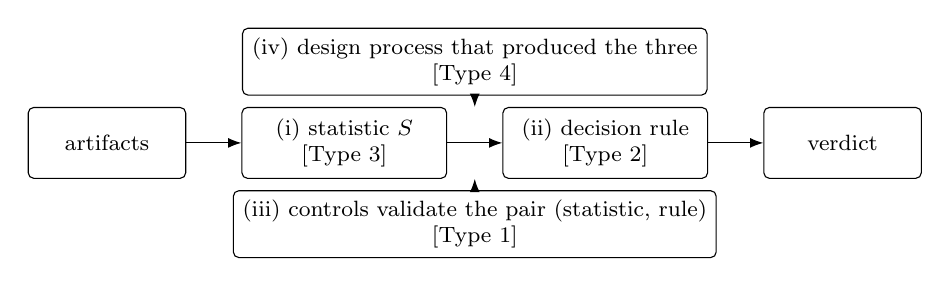
\begin{tikzpicture}[font=\footnotesize,
  box/.style={draw,rounded corners=2pt,minimum height=0.9cm,align=center},
  wide/.style={draw,rounded corners=2pt,minimum height=0.8cm,align=center}]
  \node[box,minimum width=2.0cm] (art) {artifacts};
  \node[box,minimum width=2.6cm,right=0.7cm of art] (s) {(i) statistic $S$\\{[Type 3]}};
  \node[box,minimum width=2.6cm,right=0.7cm of s] (r) {(ii) decision rule\\{[Type 2]}};
  \node[box,minimum width=2.0cm,right=0.7cm of r] (v) {verdict};
  \draw[-{Latex}] (art)--(s); \draw[-{Latex}] (s)--(r); \draw[-{Latex}] (r)--(v);
  \node[wide,below=0.6cm of $(s)!0.5!(r)$,minimum width=5.9cm] (c) {(iii) controls validate the pair (statistic, rule)\\{[Type 1]}};
  \node[wide,above=0.6cm of $(s)!0.5!(r)$,minimum width=5.9cm] (d) {(iv) design process that produced the three\\{[Type 4]}};
  \draw[-{Latex}] (c.north)--($(s.south)!0.5!(r.south)$);
  \draw[-{Latex}] (d.south)--($(s.north)!0.5!(r.north)$);
\end{tikzpicture}
\caption{Stage model of a diagnostic and where each failure mode enters. Type 1a enters at the decision rule and Type 1b at the controls. Both give the same symptom, an undecided check scored as clean.}
\label{fig:stages}
\end{figure}

\begin{definition}[Type 1, vacuous pass]
A check that did not reach a verdict is scored as clean. \emph{1a, falsy-as-clean}: the verdict function is total on a domain where $S$ is partial, so an undefined result (\texttt{nan}, \texttt{None}, an empty container) is consumed by a boolean test. \emph{1b, degenerate control}: a control whose margin to the threshold exceeds three standard deviations, or that is an identity, is counted as a true negative although it says nothing about specificity near the threshold.
\end{definition}

\begin{definition}[Type 2, structural non-discriminability]
For a case on which a diagnostic returns a verdict, the population value $\theta^\ast$ of the statistic lies close enough to the threshold $\tau$ that the flag probability at the operating audit size $n$, approximately $\Phi((\tau-\theta^\ast)/\sigma_n)$ with $\sigma_n$ the standard deviation of the audit statistic, lies between 0.05 and 0.95. For a normal statistic this means $|\tau-\theta^\ast|<1.64\,\sigma_n$. The definition describes the case and not how it was chosen. A negative control built from two implementations that a domain convention treats as interchangeable is a case of this type when their agreement sits near the threshold, as it does for detector 1. Such a control is then no clean negative.
\end{definition}

\begin{definition}[Type 3, granularity or pairing mismatch]
The aggregation level or the pairing of the statistic differs from the structure of the confound. A mismatch can only be judged against a known structure of the confound, so we give no test for it and use the term for cases where the structure was known afterwards.
\end{definition}

\begin{definition}[Type 4, post-hoc fitting]
A statistic or decision rule is changed after a failure was observed, under no change rule set before the failure.
\end{definition}

A case of Type 2 is not a malfunction of the detector. When the truth is borderline, a verdict at that audit size is close to a coin flip. The failure is a reader who takes the verdict as informative, which is why the matching reporting item asks for the flag probability at the operating audit size and not for a better threshold.

The failure modes are not complete. They leave out an invalid reference or null distribution, non-independent audit draws, plain implementation bugs, and a miscalibrated threshold that is not of Type 2, and several of these are failures inside a stage.

\paragraph{Margins and controls.} For a stochastic diagnostic with threshold $\tau$ and statistic value $s$ on a control, the margin is $m=|\tau-s|/\sigma$, with $\sigma$ the standard deviation of the statistic at the operating audit size. We fixed the following rule before computing any margin. A control is \emph{discriminating} if $m\le 3$ and a \emph{ceiling} control otherwise: it passes because it is far from the boundary, so it gives no evidence of specificity near the boundary, although it can still catch a gross bug such as a detector that always flags. At $m=3$ a control flags with probability about 0.0013. The six full-scale negative controls of detector 1 have margins 0.06, 5.39, 17.1, 33.0, 75.0 and 291, so any cutoff between 0.06 and 5.39 gives the same classification, with one discriminating control. The cutoff of 3 is a convention for a control with almost no chance of flagging and was not tuned. For example, detector 1's control that compares two windows on MIMIC-IV has kappa 0.913, a margin of 17.1, and flags with probability near zero. Margins grow with the square root of the audit size, so a ceiling control at 500 stays can discriminate at 100, and we report margins at the operating size. A large margin is expected for a positive control; the rule matters for controls counted as true negatives.

\paragraph{Estimands and scale.} Two flag probabilities appear below and are different estimands. The \emph{cohort-bootstrap} probability is the share of bootstrap resamples \citep{efron1979bootstrap} of the whole cohort whose statistic falls below the threshold. The \emph{audit-draw} probability is the share of 500-patient audit subsets drawn from the cohort that fall below it. Open-data scale means the open PhysioNet 2019 corpus and the MIMIC-IV and eICU-CRD open-data cohorts, and full scale means the full credentialed cohorts (Appendix~\ref{apd:scale}).

\paragraph{Specification and intervals.} We wrote down each experiment, its predictions and its reading rule in a committed document before it ran, and every result below was specified this way unless we call it exploratory (Appendix~\ref{apd:prereg} lists the documents). This is specification by commit order, not registration with an external registry, and commit times are author-supplied. Proportions carry exact Clopper--Pearson 95\% intervals \citep{clopper1934confidence}. Intervals on mean changes in AUROC and on the seed-level statistics of detector 2 are $t$-intervals over five seeds (four degrees of freedom), with the arms paired by seed.

\section{The Five Detectors}
\label{sec:detectors}

Detector 1 computes Cohen's $\kappa$ \citep{cohen1960kappa} on a 500-patient audit subset between two operationalizations of sepsis onset, with the Sepsis-3 criteria \citep{singer2016sepsis3} and the SOFA score \citep{vincent1996sofa} evaluated over a time window as the reference, and flags $\kappa<0.60$. Detector 2 trains a masked-reconstruction probe on a source site with a controlled share of target stays leaked in, and flags a fall in held-out target loss with a one-sided paired $t$-test over five seeds, pairing the arms by seed. Detector 3 is a static analysis of the Python syntax tree that asks whether a sweep function's evaluation call receives a loader derived from the held-out distribution. Detector 4 traces variable lineage through the same machinery to find a constraint imposed on a variable derived from it. Detector 5 compares per-component availability and a composition-controlled gap across sites. The detectors, thresholds and datasets \citep{johnson2023mimiciv,pollard2018eicu,reyna2020early,goldberger2000physiobank} did not change after the experiments in this paper were specified.

Ground truth was a real historical defect in our repository where one existed. Detector 3's positive is a buggy sweep and its fix, detector 4's is a Severinghaus circularity in our PhysioNet loader, and detector 1's is ICD-coded sepsis against SOFA scoring. Detectors 2 and 5 use controlled injection because the quantity they detect is a dose. We report per-detector counts and do not pool them, because the cases are few, heterogeneous and partly correlated (Appendix~\ref{apd:depth}).

\section{Evidence for the Failure Modes}
\label{sec:results}

Table~\ref{tab:evidence} shows how strongly each type is supported. Type 1 has the most evidence, internal and external. Type 2 is measured on one detector and illustrated, as a mechanism, on public data. Types 3 and 4 have internal evidence only.

\begin{table}[t]
\centering\footnotesize\setlength{\tabcolsep}{3pt}
\begin{tabular}{@{}lp{3.3cm}p{3.5cm}p{2.5cm}@{}}
\toprule
Type & Internal instances & External instances & Quantified by\\
\midrule
1 & five in our code (two 1a, three 1b); detector 3 returns no verdict on 53 of 53 sampled sites; the test suite passes an inverted verdict & 4 and 16 of 88 sampled sites in 25 repositories (more under an outside coder); 5 of 22 undefined cells in an executed fuzz of public checkers; one measured effect on a benchmark loader & exact intervals; control margins\\
2 & detector 1 (measured; the audit-size model holds, with one informative case); detector 5 (exploratory) & a simulation of the four-fifths rule on 133 public cases, as a mechanism that holds if audits are random subsets of 500 persons & cohort bootstrap; audit draws\\
3 & two early false negatives; one redundant gate & none & seed flag rates\\
4 & two changes made after false negatives with no change rule; one counterfactual & none & specification record\\
\bottomrule
\end{tabular}
\caption{Evidence for each failure mode. Types 3 and 4 have no external instance and rest on the same two development events.}
\label{tab:evidence}
\end{table}

\subsection{Type 1: vacuous passes}

When a check cannot reach a judgement, because the metric is undefined, the pattern is absent or the control is too easy, the outcome becomes ``no confound found'' and counts as evidence of specificity. We met this five times in our own code, in different forms (items 1 and 5 are the same pattern, an arm compared with itself, in two detectors):
\begin{enumerate}
  \item (1b) Detector 1's negative control passed the same audit array as both arguments to $\kappa$, so the result was $1.000$ by construction.
  \item (1b) Detector 1's suspicion-window controls sit at $\kappa$ from 0.91 to 1.00 across the two scales, so an external count of three true negatives implied three tests when one discriminated.
  \item (1a) Detector 3's \textsc{indeterminate} verdict on third-party repositories, folded into the true negatives, would have produced three true negatives from files it never analysed.
  \item (1a) In a baseline's train--test gap check, one seed's in-domain AUROC was undefined, the comparison of \texttt{nan} with the threshold evaluated to false, and the abstention was scored as a correct silence.
  \item (1b) Detector 2's 0\% control compares an arm with itself, so its relative change is exactly zero and the true negative holds by construction.
\end{enumerate}
Item 3 was caught before it was scored, so four of the five entered a count. Detector 1 has a latent case of the same kind: an empty audit gives a NaN kappa, the comparison with the 0.60 threshold is false, and the printout reads clean. No experiment reached it and it entered no count. The fix for all of these is mechanical: every check returns a decidability flag with its verdict, and undecidable cases go in their own column of the confusion matrix.

\paragraph{The test suite as a control.} A test suite is a control for a detector's code, and it can fail to fail, which is Type 1b one level up. We offer this as an illustration, since the mutation operators are our own and we did not use a standard tool such as mutmut. In a scratch copy we changed the check code of detectors 1 and 2 (the two files that hold their statistic, decision rule and printing) in 285 small ways: flipping or swapping comparisons, swapping boolean and arithmetic operators, removing a negation and replacing numeric constants. We ran the repository's 115 tests on each mutant. The tests failed for 29 mutants (10\%; exact 95\% interval 0.069 to 0.143) and passed for 256. Inverting detector 1's verdict, from kappa below the threshold to kappa above it, passes all 115 tests, as does setting the threshold to 0 or to 1.6. The tests check committed results and fixtures and not the live decision rule, so a low kill rate is expected, and the finding is that the suite is no control for the decision rule. Of the 285 mutants, 108 lie on verdict, test or statistic lines or on decision constants, and the tests killed 20 of them (18.5\%; interval 0.117 to 0.271); the breakdown of the rest is in Appendix~\ref{apd:mutation}. We read a random sample of 25 of the 88 survivors on those lines. Two are equivalent mutants, both entries of a critical-value table that the code never reads. The other 23 change the verdict, a statistic or a printed number for some input (share 0.74 to 0.99, so about 65 to 87 of the 88). Removing the estimated equivalents moves the kill rate on decision lines from 18.5\% to about 20\% (19\% to 24\%). Thirteen of the 23 matter only for seed counts the pipeline does not use, so 10 of the 25 sampled survivors alter behaviour on inputs the shipped pipeline can produce, two of them only at exact ties. We read those 10 as gaps in the controls and the rest as code the pipeline does not exercise.

\subsection{Type 1 in public code}
\label{sec:external}

We read 25 public repositories for the falsy-as-clean pattern: the 18 pinned repositories of Section~\ref{sec:detector3}, AI Fairness 360, and six chosen by a star-ranked rule set before any query. Almost all of this code is general-purpose machine learning, not clinical diagnostics. We froze patterns for four kinds of site before reading (236 sites) and drew 88 at random, at most two per repository and pattern group, with a seed set beforehand. A committed rubric assigned each sampled site one of guarded, unreachable, reachable and unguarded, or not applicable. The sites are code that renders verdicts, selections or aggregations and not confound detectors, so this tests the pattern and not our detectors. We did not fix in advance whether a degenerate value that arises only when training diverges counts as reachable, so we report both readings.

Under our labels the pattern is reachable and unguarded at 4 of the 88 sampled sites under the narrow reading, which counts ordinary-use sites and the divergence check itself in robustdg (exact 95\% interval 0.013 to 0.112; 3 of 88 without that check), and at 16 of 88 under the broad reading (0.108 to 0.278). The narrow positives lie in three files and three repositories, and the broad positives in 13 of 35 files and 10 of 18 repositories that contain an applicable site (Appendix~\ref{apd:positives} lists them). The sites cluster, so these intervals are descriptive; a cluster bootstrap over files gives 0.000 to 0.196 for the narrow share of applicable sites (exploratory). Per-site prevalence depends on how the frozen patterns carve code into sites, so the repository-level counts travel better. These counts describe the repositories we chose and not clinical machine learning code in general.

The counts also depend on who labels, and we have four sources of labels besides ours. Our committed labels were first produced by a language model applying the committed rubric. Four language-model raters, with our labels hidden from them, labelled the 88 sites. Their kappa with our labels is 0.63 for the rater that could read the repositories (R0, told to ignore our labels but able to read our working tree) and 0.56, 0.38 and 0.43 for three that saw excerpts only. Part of that gap is ambiguity, since the excerpt-only raters used the ambiguous label often (Appendix~\ref{apd:raters}). Three raters land near our counts (3 to 4 narrow and 13 to 17 broad of 88 sites), and one, Gemini 4 argon, is far higher (21 and 33; Figure~\ref{fig:external}). A second rater, one of the authors, agreed with us at 8 of 12 sites, but a language model corrected those labels before we recorded them, so we set it aside as evidence (Appendix~\ref{apd:raters}).

\begin{figure}[t]
\centering
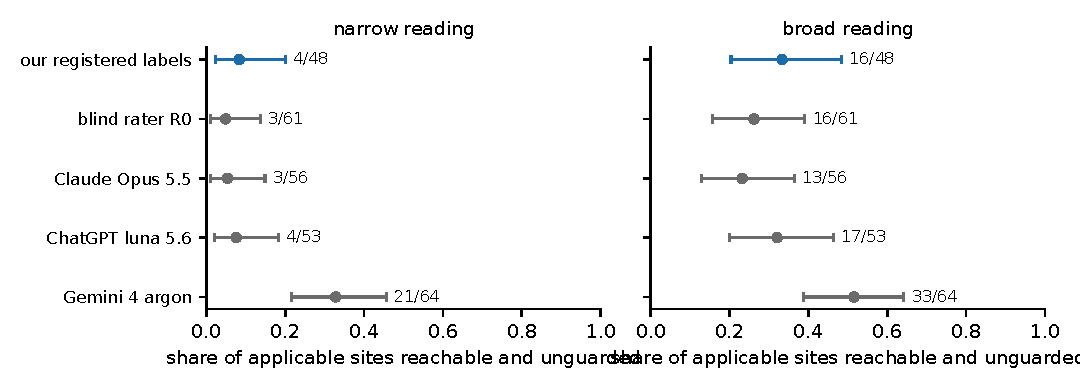
\includegraphics[width=0.98\linewidth]{figs/fig4_external.pdf}
\caption{Sites reachable and unguarded for the falsy-as-clean pattern, out of the 88 sampled sites, under our labels, four language-model raters and an outside human coder. The raters' narrow counts exclude the divergence check that ours includes. Blue and grey points carry exact 95\% intervals. The coder labelled 40 sites, so the coder's point is scaled to 88 with a within-stratum bootstrap interval. The narrow reading excludes sites whose degenerate value arises only in diverged training.}
\label{fig:external}
\end{figure}

An outside human coder with Python and machine-learning experience, using no language model for the labelling, labelled 40 of the 88 sites from the committed rubric with our labels hidden. The sample was fixed beforehand: all 16 sites counted under the broad reading, 12 of the other 32 applicable sites and 12 of the 40 not-applicable sites. The coder agreed with us on 15 of the 16 broad positives (exact interval 0.70 to 1.00), 8 of 12 other applicable sites (0.35 to 0.90) and 4 of 12 not-applicable sites (0.10 to 0.65). Because the first stratum is all of our positives, the 15 of 16 measures the precision of our positives and not their recall, and the weak agreement in the other two strata is where recall shows. Weighted by stratum size, kappa on the four labels is 0.42 (bootstrap interval 0.23 to 0.64), below our line of 0.60, and the labels are rubric-dependent here as well. On the one question that carries the counts, whether a site is reachable and unguarded under the broad reading or not, kappa is 0.62, above our line of 0.60, so most of the disagreement is about which no-failure label applies. The disagreements run toward more positives. Scaled to the 88 sites, the coder's labels give about 26 reachable and unguarded sites under the broad reading (bootstrap interval 18 to 38) and about 14 under the narrow one (6 to 26), against our 16 and 4, so our 4 may be an undercount under the coder's reading. Our own second reading of the five sites where we and the coder differ, which we made ourselves, keeps one positive and moves the other four to undecidable or unreachable (Appendix~\ref{apd:raters}). The scaled counts therefore rest on about four contested sites, each weighted about three times. The pattern exists, and its rate has no stable estimate. The coder used a language model only to reformat the coder's own notes into the response file, and the labels in that file match the coder's original document. One coder is a thin sample.

\paragraph{Executed behaviour.} Three public codebases behave as the pattern predicts on inputs we ran. The tableshift College Scorecard task \citep{gardner2023tableshift} maps the completion-rate target with a comparison against 0.5 followed by \texttt{astype(int)}, and its configuration turns row dropping off, so a missing target becomes the label 0. The benchmark's own data file needs a login, so we ran the verbatim function on the official most-recent institution file \citep{collegescorecard}. Of 6,272 institutions, 3,994 (63.7\%) have no completion rate. The line turns them into negatives and moves the positive share from 0.521 among observed rows to 0.189 overall. We compared this with a guarded pipeline that drops the missing-target rows, using the same features, five random 70/30 splits and a gradient-boosted classifier trained by us as a stand-in for the benchmark's own models. The unguarded pipeline reports an AUROC 7.6 points higher than the guarded one reports ($t$-interval 6.8 to 8.5) and an accuracy 12.3 points higher (11.5 to 13.0). Scored against true labels on the observed-target test rows, the unguarded-trained model is slightly worse, by 1.5 AUROC points (0.8 to 2.2 lower). We predicted both directions beforehand. The unguarded pipeline would report an AUROC more than 0.02 higher than the guarded one (observed 0.076), and the unguarded-trained model would not beat the guarded one on true labels by more than 0.01 AUROC (observed difference $-0.015$, so it is worse). Both predictions held. The reported accuracy gap also mixes the label change with a base-rate change (majority-class accuracy 0.811 against 0.518), which is why we lead with AUROC; an exploratory check gives balanced accuracy 6.4 points higher (4.9 to 7.9). The line raises the reported numbers without making the model better. This is the effect of the line on the official file with a stand-in model. Reachability is inferred from the dataset's missing-value settings and was not executed on the benchmark's own file, which could differ from the 2026 official file we used. The five random splits overlap, so the intervals are optimistic, and they are not the benchmark's distribution-shift splits, so the effect on its reported numbers is unknown. Running the benchmark's own file would turn the inference into a measurement.

The other two behaviours change a count or a check and not a reported metric. In fairseq2, the range filter and list-length filter keep null-list rows when no other row fails and drop them otherwise (a table of 10,000 rows with 1\% null lists gives 10,000 rows, or 9,907 once one failing row is added). In robustdg, the divergence check takes the maximum of the training and test losses and then tests whether it is finite, so a NaN test loss with a finite training loss goes unnoticed. Both are properties of the code on the inputs it receives and not reports of an incident (Appendix~\ref{apd:d2detail}). The selection and guard lines of DomainBed \citep{gulrajani2021search} accept a NaN score listed first and an empty list on synthetic inputs, but the shipped datasets cannot reach those inputs.

\paragraph{An executed fuzz of public checkers.} We ran 13 built-in checks from Great Expectations 0.18.22, pandera 0.35.0, Fairlearn 0.15.0, AI Fairness 360 0.6.1 and scikit-learn 1.9.1 on a nominal table, where all 13 behaved, and on seven degenerate tables (empty, all NaN, constant, single class, one row, single group and infinite). Of the 91 cells, 23 had a statistic that a mapping fixed before the run called undefined. In those 23, 9 raised an error, 5 failed, 3 returned NaN and 6 passed or returned a finite value without a warning. One of the six, scikit-learn's kappa for a constant reference rater, is defined on its input, so our mapping was wrong for that cell. The corrected result is 5 of 22 cells (exact interval 0.078 to 0.454), from 4 of the 13 checks (0.091 to 0.614); we use the check as the unit because the cells of one check are correlated. Appendix Table~\ref{tab:fuzzcells} lists the five. Three are conventions, since a universal check on an empty column passes vacuously, one is arguably defined (a single group is trivially at parity), and one is undefined (a false-positive rate with no negatives). The docstrings of the pinned versions, which we read without running them, are silent on what these checks do on such input, and we read no user guides. The result is behaviour on degenerate input that the docstrings leave open, and it is no finding that a tool is wrong.

\subsection{Type 2: a statistic on its threshold}
\label{sec:type2}

On full MIMIC-IV the whole-cohort $\kappa$ between SOFA window and single-point scoring, two defensible operationalizations of Sepsis-3, is $0.602$ (cohort-bootstrap 95\% interval 0.597 to 0.607). That is 0.002 above the 0.60 cutoff and 0.06 standard deviations of the 500-patient audit-draw distribution from it, so a 500-patient audit flags 48.4\% of the time. The same pair gives $0.826$ on eICU-CRD, a ceiling control ($m=5.39$). Variation across databases (0.224) is large next to the 0.002 by which the MIMIC-IV control clears the threshold. By the margin rule that control is the only one of six full-scale negative controls that discriminates. The positive cases sit at $m=12.13$ (MIMIC-IV) and $m=2.59$ (eICU-CRD). Across the six negative pairs the whole-cohort kappa is 0.60, 0.91 and 0.99 on MIMIC-IV and 0.83, 0.99 and 1.00 on eICU-CRD.

The control is therefore not a clean negative: two implementations that a domain treats as interchangeable agree at 0.602, so they are less interchangeable than the convention suggests, and the next paragraph shows that this holds for one contrast only. The 500-patient audit is the shipped detector's operating point and not a recommendation. If both operationalizations can be computed on the whole cohort, the verdict is deterministic (0.602 does not flag), so this Type 2 case comes from the subset audit design together with a threshold taken from convention.

\paragraph{How special is the coincidence?} We relabelled both cohorts under ten operationalizations of Sepsis-3 that differ only in the window of the SOFA score around the suspected infection (24, 48 or 72 hours before and 12, 24 or 48 hours after it), plus the single-point rule, and computed the whole-cohort kappa for all 45 pairs. The four variants we had already used reproduce the stored labels for every stay in both databases. On MIMIC-IV, 6 of the 45 pairs have a 500-patient flag probability between 0.05 and 0.95 (exact interval 0.051 to 0.268) and 9 have $m\le 3$. All six are the single-point rule against a window, with kappa from 0.55 to 0.61, and no pair of two windows is near the threshold (kappa 0.85 to 0.99 for 36 pairs). On eICU-CRD none of the 45 is (0 of 45, 0.000 to 0.079; kappa 0.82 to 1.00). We predicted that fewer than 10\% of pairs would sit in the zone. The prediction missed on MIMIC-IV, where 6 of 45 (13\%) do, although the interval includes 0.10, and it held on eICU-CRD. Sitting on the threshold is therefore a property of one contrast, single-point against windowed scoring, in one database. The 45 pairs share variants and the family is our choice, so the interval describes this family and not operationalizations in general. The suspicion rule, the look-back and the SOFA threshold are the same across the family.

Two flag probabilities are easy to conflate here. The value 0.216 at open-data scale is a cohort-bootstrap value on 117 stays, and 0.484 at full scale is an audit-draw value on 74,829, so the rise between them is not a trend. Like for like, the cohort-bootstrap probability is 0.216 at open-data scale and 0.241 at full scale.

\paragraph{Does the model predict other audit sizes?} The Type 2 model takes the whole-cohort $\theta^\ast$ and the audit-draw standard deviation at $n=500$, rescales the latter to other sizes with a finite-population correction, and predicts the flag rate. We fixed the predictions, the sizes and a reading rule beforehand: a maximum absolute deviation of 0.05 or less over $n\in\{200,500,1000,2000\}$ counts as support. With 2,000 audit subsets per size and case, the model matched the simulated audit draws within the 0.05 band in all three cases (maximum deviation 0.026 for the MIMIC-IV control, 0.010 for the eICU-CRD positive and 0.004 for the eICU-CRD control; Figure~\ref{fig:audit}). Only the MIMIC-IV control is a real test, because the eICU-CRD cases sit far from the threshold, where flag rates near 0 or 1 are easy to predict. The standard deviation was taken at $n=500$, so that size is not a held-out test, and the model is close to a normal approximation with a finite-population correction. For the MIMIC-IV control the observed flag rate falls only from 0.492 at $n=100$ to 0.411 at $n=5{,}000$. The model puts the audit size at which the verdict would settle, with a flag probability below 0.05 or above 0.95, at 62,500 of the 74,829 stays, so no audit of a practical size resolves this verdict. The finding is about the position of the threshold and not about the sample.

\begin{figure}[t]
\centering
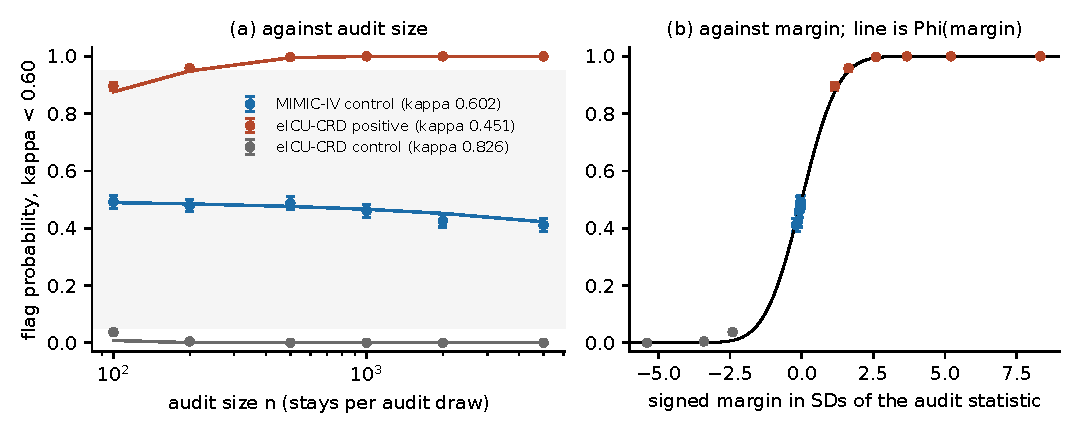
\includegraphics[width=0.98\linewidth]{figs/fig2_audit_size.pdf}
\caption{Flag probability of detector 1 on full-scale labels. Points are observed rates over 2,000 audit draws with exact 95\% intervals, and lines are the Type 2 model fixed before the run. (a) Against audit size: the MIMIC-IV control stays between 0.41 and 0.49 for every size from 100 to 5,000 stays, and the shaded band marks flag probabilities between 0.05 and 0.95. (b) The same 18 points against the signed margin of the threshold from the population value, in standard deviations of the audit statistic; the model curve is the normal distribution function.}
\label{fig:audit}
\end{figure}

We left the threshold where it was, because moving it would be Type 4. The 0.60 value is a convention with no clinical derivation, and conventions for kappa differ \citep{mchugh2012kappa}. For new detectors, a negative control should be a pair of implementations that a domain expert accepts as interchangeable, and the threshold should sit clear of the spread of the statistic across such pairs. This is a prescription fixed before looking at data.

\paragraph{A second instance (exploratory).} Detector 5's composition ratio, a ratio of two gaps that a normal approximation describes poorly, on PhysioNet Site A against Site B has a gate at 0.30. Over five seeds at 1,200 stays per arm its mean is 0.283 (SD 0.082) and it flagged 2 of 5; at 4,000 stays the mean is 0.272 (SD 0.027) and it flagged 0 of 5; at 900 and 1,500 stays it flagged 3 of 5. A normal approximation fitted to the five seeds gave flag probabilities of 0.42 and 0.15 at 1,200 and 4,000 stays. We tested this on 20 fresh seeds at both sizes. At 1,200 stays 13 of 20 flagged (exact interval 0.408 to 0.846), and the predicted 0.42 lies inside it, barely. At 4,000 stays 8 of 20 flagged (0.191 to 0.640), and the predicted 0.15 lies outside it, so the prediction failed there. The fresh ratios were more variable than the first five seeds suggested (SD 0.145 against 0.082 at 1,200 stays, and 0.055 against 0.027 at 4,000), so five seeds were too few to fit the spread. At 4,000 stays, more than three times the data, detector 5 still flags 40\% of the time. The same-site control flagged in none of the 40 fresh runs (0 of 20 at each size; interval 0.000 to 0.168).

\paragraph{A simulation on public data (exploratory).} The four-fifths rule gives a second view of the mechanism. We applied it to 133 public cases (the American Community Survey \citep{ding2021retiring}, UCI Adult \citep{ucicadult} and COMPAS \citep{angwin2016machinebias}) and drew 2,000 audits of 500 persons per case. The flag rate lay between 0.05 and 0.95 in 93 of 133 cases (0.614 to 0.776), but this says mostly that a 500-person audit of a ratio is noisy. If the population ratios were placed at random over their observed range with each case keeping its own audit standard deviation, we would expect 77 to 80 cases within 1.64 standard deviations of the threshold, and we observe 77. The cases are no closer to the threshold than chance placement predicts. The comparison is weak evidence either way, since uniform placement is an assumption we leave undefended, and it does not test whether the rule is calibrated. The cases show audit noise. This holds only if audits are random subsets of 500 persons, an assumption we leave undefended (Appendix~\ref{apd:fourfifths}).

\subsection{Types 3 and 4: two hazards from our development}

We have no measurement of these two types. Both rest on the same two events in our own development: detector 5 aggregated at the wrong granularity, and detector 2 compared unpaired where the comparison is paired (Type 3). Both changes followed a false negative under no change rule set beforehand (Type 4), and the repository history does not date them. Pre-specification prevented one further change, a counterfactual. We present both types as hazards that can arise in a development process like ours and not as measured instances. Appendix~\ref{apd:hazards} gives the full account.

\subsection{Detector 2: a control that holds corpus size fixed}
\label{sec:detector2}

Detector 2 serves here as a vehicle for the audit and is not a contribution. Its 0\% control cannot show a corpus-size effect, because it holds the corpus fixed. We added an arm (A2) that adds extra \emph{source} stays in place of target stays. Let $r_1$ be the shipped detector's mean relative reduction in probe loss and $r_2$ that of A2. The ratio $r_2/r_1$ (Figure~\ref{fig:volume}) is 0.31 and 0.48 at 5\% and 20\% leakage on the PhysioNet pair at open-data scale, and 0.55 and 0.69 at full scale on MIMIC-IV to eICU-CRD. Both full-scale values are above our line of 0.5, so by our own rule corpus size confounds the effect. With five seeds the ratios are imprecise. Fieller 95\% intervals (exploratory) are $-1.32$ to 0.64 and 0.38 to 0.61 on the open-data pair, and $-0.86$ to 0.78 and 0.55 to 0.78 at full scale, so only the full-scale 20\% ratio is clearly above 0.5, and we read the full-scale 5\% case as undetermined. Target exposure still adds beyond volume (shipped arm against A2, paired $t=9.0$ and 15.4 at full scale). The result is narrower than the shipped statistic alone suggests.

\begin{figure}[t]
\centering
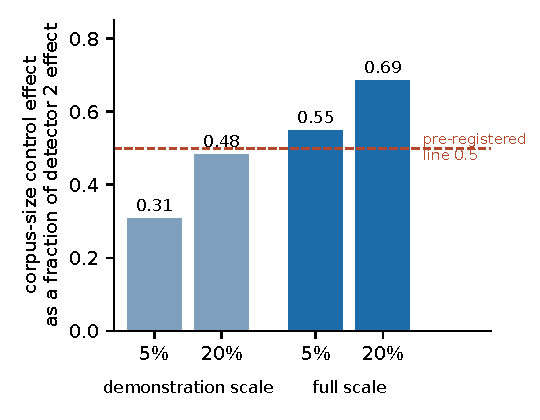
\includegraphics[width=0.52\linewidth]{figs/fig3_volume_control.pdf}
\caption{Effect of the corpus-size control (A2) as a fraction of the effect of detector 2 (arm A1), by leakage level and scale, five seeds. Both full-scale bars exceed our line of 0.5, but only the 20\% bar has an interval (0.55 to 0.78) that excludes it. Error bars are Fieller 95\% intervals (exploratory), and a triangle marks an interval that extends below 0.}
\label{fig:volume}
\end{figure}

A null of 20 independent paired five-seed comparisons of two no-leak arms, each with a fresh data draw and model seed, flagged 1 of 20 (exact interval 0.001 to 0.249; exploratory). That agrees with the nominal 5\% and is a harder test than the detector's own shared-seed comparison. Detector 2's dose sweeps, missingness arms and baselines are in Appendix~\ref{apd:fullscale}. The shipped statistic first flags at 5\% leakage at both scales. A volume-matched statistic also flags at 1\% and 2\%, where the corpus-size arm is within 0.005 of zero, and that is no evidence of a lower detection floor. At full scale the arms that split target values from target observation pattern (A3 and A4; A1 is the shipped detector) read as mixed: the share carried by the observation pattern is 0.22 and 0.30, and the mask-transplant difference clears the critical value at 5\% only. Several of these readings sit close to their thresholds ($t=1.94$ against 2.132 at 2\% for the shipped statistic, and 2.58 against 2.132 for the 5\% mask comparison), and a rerun on a second CPU shifted $t$ by up to about 0.5 with the same flags and verdicts, although the 5\% and 20\% shipped and corpus-size runs were not retrained there. Another machine could therefore have flipped them. Standard checks carry no information about detector 2's scenario, and leakage moves cross-site AUROC by at most about 0.007 at open-data scale (exploratory), and the full-scale intervals reach $-0.018$ to $+0.013$, so the practical importance of what detector 2 measures remains open.

\subsection{Detector 3 outside its home idiom}
\label{sec:detector3}

Over 18 pinned public repositories, each linked to a paper (735 Python files, 727 parsed and 8 unparseable), detector 3 recognised a sweep in none, with its shipped vocabulary and with one fitted to those repositories. To get a denominator we enumerated candidate selection sites with patterns frozen before the scan: 103 sites in the 688 non-test files, 680 of which parse. We sampled 53 and labelled each with a rubric committed before any site was read and before the detector ran. By those labels none was contaminated: one was a disclosed oracle, one was ambiguous, 21 were sound and 30 were not selections, so undisclosed contamination was absent from 0 of 23 real selection sites (exact interval 0.000 to 0.148). The model raters disagreed with these labels (kappa 0.64, 0.59, 0.28 and 0.22 across the four), and the disagreements that matter concern contamination. After rereading, we judge one site contaminated and our committed label wrong: a hyperparameter sweep in robustdg picks the best configuration by a value its comment calls source validation accuracy, which is the test-domain accuracy at the epoch chosen by source validation. Two more sites are unresolved. Undisclosed contamination is then present in 1 of 23 real selection sites (0.001 to 0.219), or 3 of 24 (0.027 to 0.324) if the two unresolved sites count (one of them was labelled not a selection, so counting it also adds it to the denominator). Detector 3 returned \textsc{indeterminate} on the files of all 53 sites, so it missed every contaminated site and issues no clean verdict. Its sensitivity is 0 of 1 to 0 of 3, which is defined but uninformative, and we describe it as a guard for one's own sweeps and not a retrospective auditor. The scan covers Python files only, and 126 notebooks were not scanned.

We also built the tool of \citet{yang2022leakage} in Docker after three changes to its build environment and ran it on detector 3's buggy and corrected fixtures. It reports zero in each of its three categories (overlap, pre-processing, multi-test) on both. The fixtures are not in the format the tool targets, so this shows that it does not apply to our idiom and not that it fails in general. We found no baseline for detector 4 in two literature searches, which is a thin basis. Detector 5's natural baseline is the cross-site gap it decomposes, which is an input and not an independent check, so we ran none.

\section{A Reporting Standard for Diagnostics}
\label{sec:standard}

The failures above suggest five items to report with a diagnostic's verdict. Items 1 to 4 come from failures we measured and item 5 from the hazard in our development. None needs new data except the replicate runs of item 4.
\begin{enumerate}
  \item \textbf{A decidability flag.} Every check returns whether it reached a verdict, and undecidable cases are counted separately from clean ones (Type 1a).
  \item \textbf{Control margins.} Report $m=|\tau-s|/\sigma$ for every control, and do not count a ceiling control or an identity as a true negative (Type 1b).
  \item \textbf{Uncertainty at the operating point.} Report the flag probability at the audit size actually used, and the audit size at which the verdict would settle (Type 2; Figure~\ref{fig:audit}).
  \item \textbf{A null rate and a nuisance control.} Run independent replicates of the no-effect comparison, and a control that holds the diagnostic's nuisance variables, such as corpus size, apart from the confound (Section~\ref{sec:detector2}). This item asks for two things that we found together.
  \item \textbf{Provenance of the decision rule.} Set the rule before the data, and say so if it changed afterwards (Type 4).
\end{enumerate}
These items address Types 1, 2 and 4 and the nuisance-control part of the corpus-size finding. We have no item for Type 3. Items 1 and 3 can be combined into a three-way verdict of flag, clear or inconclusive, where inconclusive covers an undecided check and a flag probability between 0.05 and 0.95 at the audit size; we did not compare this with flagging only when a confidence interval clears the threshold. We derived the items from our own cases and mapped them to those cases after the results (Appendix~\ref{apd:standard}), so the standard has no test beyond them. Appendix~\ref{apd:standard} also fills it in for detector 1.

\section{Limitations}
\label{sec:limits}

\paragraph{Circularity.} The same group built and audited every detector, and the external counts depend on labels that began with a language model. The labelling by raters, a second rater and one outside human coder narrows this and does not remove it. The model raters share training with the model that wrote our first labels, one of them could read our working tree, and their median kappa was below our line. The outside coder labelled 40 of the 88 reachability sites and none of the 53 model-selection sites, and kappa was 0.42 on four labels. Independent coding of all 141 sampled sites by more than one person outside the group would resolve this.

\paragraph{Uneven evidence.} We did not apply the margin and decidability checks to other groups' published diagnostics, so the evidence is about our five detectors. Types 3 and 4 rest on the same two development events and have no external instance. Type 2 rests on one detector, on one contrast in one of two databases, with detector 5 as an exploratory second whose model, fitted on five seeds, failed its prediction at one of two sizes. The four-fifths cases hold only if audits are random subsets of 500 persons. Outside instances of Types 2, 3 and 4 in other groups' diagnostics would resolve this.

\paragraph{Limited demonstrated consequence.} We show a pattern in other groups' code, with 4 and 16 of 88 sampled sites under our labels, a measured effect at one of the four narrow positives on the official College Scorecard file with a stand-in model, and executed behaviour at two more. No site is shown to have changed a published conclusion, and the DomainBed lines cannot be reached with the shipped datasets. Running the tableshift line on the benchmark's own file would resolve the first gap, and finding a study that used one of the other sites would resolve the second. The repositories are general-purpose machine learning code, so the clinical scope of the title rests on our own detectors.

\paragraph{Small internal suite and seed counts.} Appendix Table~\ref{tab:depth} has denominators of 1 to 8 and says nothing about performance elsewhere. Most seed-level results use five seeds, and the fresh-seed test of detector 5 showed that five seeds can understate spread by a factor of two. We did not rerun the near-threshold cases of detector 2 with more seeds.

\paragraph{Detector limits and definitions.} Corpus size confounds detector 2's effect at full scale, and its missingness arms read as mixed with five seeds and a small model. Detector 3 has no demonstrated sensitivity outside its home idiom. Detector 5's external component set is analogous and not identical. The full-scale detector 2 runs use caches of 74,607 and 130,446 stays, which differ slightly from the cohorts used for detector 1. We wrote the definitions of the failure modes ourselves, and review by clinicians and verification researchers would test them.

\section{Conclusion}
\label{sec:conclusion}

A clean confusion matrix does not tell a reader whether a diagnostic could have failed. Auditing five of our own detectors gave four failure modes with evidence of different strength. Type 1 is best supported. Type 2 is measured on one detector, with a model that predicted held-out audit sizes, and shows the same audit noise in public data if audits are random subsets of 500 persons. Types 3 and 4 are hazards from our own development. We recommend that every diagnostic have an undecidable state, report control margins and the flag probability at the audit size used, and fix its decision rule first. Whether the failures we found in our own tools change conclusions in other groups' work is still open.

% Use of language models: statement left blank for the owner to write.

\paragraph{Broader impact.} The work uses de-identified, credentialed critical-care data under their data-use agreements. Only aggregate results are released, and per-stay arrays are not.

\bibliographystyle{tmlr}
\bibliography{ref}

\appendix
\section{Reproduction}
\label{apd:repro}
The test suite has 115 tests, which check committed results and fixtures (Section~\ref{sec:results} shows what they do not catch). With the PhysioNet and demonstration data present all 115 pass. Without them 108 pass and 7 skip with the reason \texttt{PhysioNet data not present}, because a test that cannot run has not succeeded. The release contains the detector code, the specification documents and every aggregate result. Per-stay arrays derived from MIMIC-IV and eICU-CRD are not released.

\section{Specification documents}
\label{apd:prereg}
Each experiment was specified in a committed document before it ran. Addenda 1 to 3 of the first set precede the experiments in the main text. The later addenda were written after the results of earlier experiments and specify later ones. Commit times are author-supplied metadata, so the hashes are the check, and the release carries a manifest of the SHA-256 of each document at its commit. Table~\ref{tab:spec} lists them, and Table~\ref{tab:status} gives the status of each result.

Deviations from the specifications are few. The consequence study and the fuzz each have a document that records changes to their tools and checks (8252b06 and 64a5ed0). The outside-coder document was corrected before the sample was drawn. We added a bootstrap for the scaled counts of the outside coder after the labels were in, and our second reading of the five contested sites came after them. Our fuzz mapping was wrong for one cell (scikit-learn's kappa), which we report as a correction. The volume-matched statistic at 1\% and 2\% was read beyond the rule we had written, which covered only the doses where the shipped statistic flags. Several analyses were added after seeing results and are labelled exploratory in the text. We applied no multiplicity adjustment to the intervals, and about 20 specification documents lie behind the results.

\begin{table}[h]
\centering\footnotesize
\begin{tabular}{@{}p{5.0cm}p{3.7cm}p{3.7cm}@{}}
\toprule
Experiments & Commit & SHA-256 (first 12)\\
\midrule
Detector 5 variant rule, then the code using it (29 minutes apart) & 63f5d95a8a8e, 1600d91071cf & \\
Ablation and corpus-size experiments (main document, site patterns and rubrics, addenda 2, 3, 3b) & 25fc617, b845cc0, 4c461eb, bc365cf, 073d042, 879d885, d14687a, 4918770, 69148a9 & \\
Audit-size and fresh-seed predictions & 829a11c & 49cabc337b70\\
Four-fifths, consequence and fuzz experiments; their deviations and tools & 15042cb, 8252b06, 64a5ed0 & 3fc4bdd22e56, d95b11a8800b, c1f4606e442f\\
Label-masked language-model raters; three external raters and reading rule & 3e12272, 6afd129 & fe257c4b7167, 0b91699199f7\\
Dose sweep and mutation test (scripts in a0377f4, db04005) & 583d357 & 242520918888\\
Sepsis-3 operationalization family, full-scale missingness arms and dose sweep (scripts in 3981dc0) & 56d835d & fa2d0eb4a353\\
Guarded-pipeline comparison and equivalence sample of mutation survivors & 6292d3b & 4aececcef9ef\\
Outside human coder (corrected before the sample was drawn) & f42b84e, da3dc41 & \\
\bottomrule
\end{tabular}
\caption{Documents that fix each experiment before it ran.}
\label{tab:spec}
\end{table}

\section{Scales and cohorts}
\label{apd:scale}
Open-data scale means the open PhysioNet 2019 corpus and the MIMIC-IV and eICU-CRD demonstration cohorts, with 117 and 1,627 stays. Full scale means MIMIC-IV ($n=74{,}829$) and eICU-CRD ($n=132{,}900$) for detector 1, and the slightly smaller extracted cohorts of 74,607 and 130,446 stays for detector 2 and its baselines. At open-data scale detector 2 draws 900 nominal stays per site, and the loader's filters leave 602 to 651 source stays. Detector 5 uses 1,200 stays per arm unless a size is given.

\section{Detector 1 controls}
\label{apd:controls}
\begin{table}[h]
\centering\footnotesize
\begin{tabular}{@{}llccl@{}}
\toprule
Database & Control (SOFA window against) & $\kappa$ & Margin $m$ & Class\\
\midrule
MIMIC-IV & single-point & 0.602 & 0.06 & discriminating\\
MIMIC-IV & window $[-24,+12]$ & 0.913 & 17.1 & ceiling\\
MIMIC-IV & window $[-72,+24]$ & 0.993 & 75.0 & ceiling\\
eICU-CRD & single-point & 0.826 & 5.39 & ceiling\\
eICU-CRD & window $[-24,+12]$ & 0.986 & 33.0 & ceiling\\
eICU-CRD & window $[-72,+24]$ & 1.000 & 291 & ceiling\\
\midrule
MIMIC-IV & ICD-coded sepsis (positive) & 0.174 & 12.13 & ceiling\\
eICU-CRD & ICD-coded sepsis (positive) & 0.451 & 2.59 & discriminating\\
\bottomrule
\end{tabular}
\caption{Full-scale controls of detector 1 against the reference window $[-48,+24]$, with the whole-cohort kappa, the margin at 500 patients and the class by the margin rule. The window-against-window rows are the suspicion-window controls of item 2 in Section~\ref{sec:results}. The identity control of item 1 passed one array twice, so its kappa of 1.000 held by construction, and it is not in this table. A large margin is expected for a positive control.}
\label{tab:controls}
\end{table}

\section{Status of each result}
\label{apd:status}
\begin{table}[h]
\centering\footnotesize
\begin{tabular}{@{}p{5.2cm}p{7.6cm}@{}}
\toprule
Status & Results\\
\midrule
Specified before the run & mutation test and the sample of survivors; the 25-repository read (patterns, rubric; the divergence convention was not fixed); label-masked raters and the outside coder; the fuzz; the loader comparison; the 45-pair family; the audit-size model; the fresh-seed test of detector 5; the corpus-size arm; the dose sweeps; the missingness arms; the scan of detector 3; the four-fifths simulation\\
Exploratory & triage of survivors by role; cluster bootstrap over files; Fieller intervals; the base-rate check on the loader; the restricted-size and reference-rate analyses of the four-fifths cases; the null of 20 comparisons; the downstream change; our second reading of the contested sites; the scaling of the outside coder's counts\\
Descriptive & the five internal Type 1 cases; the two development events behind Types 3 and 4\\
\bottomrule
\end{tabular}
\caption{Status of each result. Specification is by commit order and not an external registry.}
\label{tab:status}
\end{table}

\section{Type 1 positives}
\label{apd:positives}
Reachable and unguarded under the narrow reading (repository, file, line, pinned commit): tableshift, \texttt{tableshift/datasets/college\_scorecard.py}:170, \texttt{fca9429814} (a NaN target becomes 0, and the task's configuration keeps such rows; reachability inferred from the dataset's missing-value settings); fairseq2, \texttt{src/fairseq2/data/parquet/arrow\_transform.py}:288 and :306, \texttt{7f06d6f4f5} (null rows pass a length filter); robustdg, \texttt{utils/scripts/utils.py}:579, \texttt{3eee1730ae} (a \texttt{max} of two losses returns the finite one when the other is NaN, which defeats the \texttt{isfinite} check on the next line). \pending{Responsible disclosure: record the date maintainers were notified before submission.} Table~\ref{tab:external} splits the sites by kind of code.

\begin{table}[h]
\centering\footnotesize
\begin{tabular}{@{}lccc@{}}
\toprule
Reading & Verdict or selection code & Other code & All applicable sites\\
\midrule
Narrow & 1/27 [0.001, 0.190] & 3/21 [0.030, 0.363] & 4/48 [0.023, 0.200]\\
Broad & 11/27 [0.224, 0.612] & 5/21 [0.082, 0.472] & 16/48 [0.204, 0.484]\\
\bottomrule
\end{tabular}
\caption{Reachable and unguarded sites among applicable sampled sites, with exact 95\% intervals; the denominators are applicable sites, which depend on the labeller. Fisher exact tests of verdict or selection code against other code give $p=0.31$ (narrow) and $p=0.35$ (broad). The direction reverses with the convention, so we found no evidence that the pattern concentrates in code that renders verdicts.}
\label{tab:external}
\end{table}

\section{Raters and the outside coder}
\label{apd:raters}

\paragraph{Second rater.} A second rater, one of the authors, labelled 12 randomly drawn sites (six per rubric) on 2026-10-10 from the committed rubrics, without seeing our labels. The rater then gave the labels and a short description of the task to a language model (Claude Sonnet 5), which checked them for errors and corrected the ones it flagged. The record holds only the corrected labels, so agreement before the model check is not available. The final labels agreed with ours at 8 of 12 sites (exact interval 0.349 to 0.901).

\paragraph{Language-model raters.} Four language-model raters labelled the 53 model-selection sites and the 88 reachability sites from sheets that hid our labels. Our labels were hidden from each rater, but the raters share training with the model that wrote our first labels. One rater could read the pinned repositories (R0, a Claude model run inside our session) and also had read access to our working tree, where the label files were stored, so its blindness rests on its instructions. Three saw only the matched lines with up to 30 lines of context on each side: Claude Opus 5.5 at high effort, Gemini 4 argon at medium thinking and ChatGPT luna 5.6 in thinking mode, each in a fresh chat on 2026-11-11, with the model and setting names taken from the recorded file names. Table~\ref{tab:raters} gives agreement with our labels. The median kappa across the four raters is 0.43 on the model-selection sheet and 0.50 on the reachability sheet, and without R0 it is 0.28 and 0.43, all below our line of 0.60.

\begin{table}[h]
\centering\footnotesize\setlength{\tabcolsep}{4pt}
\begin{tabular}{@{}lcccc@{}}
\toprule
 & \multicolumn{2}{c}{Model selection (53 sites)} & \multicolumn{2}{c}{Reachability (88 sites)}\\
Rater & agree [95\% CI] & $\kappa$ & agree [95\% CI] & $\kappa$\\
\midrule
R0 (told to ignore labels) & 42 [0.659, 0.892] & 0.64 & 64 [0.622, 0.817] & 0.63\\
Claude Opus 5.5, high & 39 [0.597, 0.847] & 0.59 & 60 [0.574, 0.777] & 0.56\\
Gemini 4 argon, medium & 25 [0.333, 0.614] & 0.28 & 45 [0.403, 0.620] & 0.38\\
ChatGPT luna 5.6, think & 23 [0.298, 0.577] & 0.22 & 52 [0.481, 0.695] & 0.43\\
\bottomrule
\end{tabular}
\caption{Agreement of four language-model raters with our labels, as the count of agreeing sites with its exact 95\% interval and Cohen's $\kappa$. The three raters that saw only excerpts give the lowest values.}
\label{tab:raters}
\end{table}

The excerpt-only raters chose the ambiguous label far more often on the model-selection sheet (25 of 53 for Gemini and ChatGPT, 12 for Claude Opus, against 2 for R0), as the rubric tells them to when the excerpt does not settle the question. On the sites where a rater gave a definite label and we did too, agreement was 41 of 51 for R0 ($\kappa=0.64$), 38 of 41 for Claude Opus (0.86), 25 of 27 for Gemini (0.82) and 23 of 27 for ChatGPT (0.49); this reading is exploratory. On the model-selection sheet the raters found 1 or 2 contaminated sites among 30 to 33 real selection sites, against none among 23 in our labels. On the reachability sheet the narrow counts are 3 of 61 applicable sites (R0), 3 of 56 (Claude Opus), 4 of 53 (ChatGPT) and 21 of 64 (Gemini, which labelled many sites reachable in ordinary use), and the broad counts are 16 of 61, 13 of 56, 17 of 53 and 33 of 64.

\paragraph{Our reading of the sites where raters disagreed.} We read the sites where most raters disagreed with us on a headline count. In robustdg, the sweep in \texttt{slab-tune.py} lines 85 to 88 picks the best file by a value its comment calls source validation accuracy, which \texttt{train.py} prints as the test-domain accuracy at the epoch chosen by source validation. We judge it contaminated and our committed label wrong. We leave two sites unresolved: eICU-GNN-LSTM \texttt{train\_ns\_lstmgnn.py} line 179 has what look like swapped validation and test masks, and robustdg \texttt{utils.py} lines 362 to 364 chooses a checkpoint by an error on the test loader. robustdg \texttt{train.py} line 303 is the disclosed oracle we already count separately. On reachability, wilds \texttt{all\_metrics.py} line 152 was committed not applicable and all four raters called it reachable. We agree, since NaN scores compare false and their boxes are dropped without a message, and it counts under the broad reading only. robustdg \texttt{ptb\_utils.py} line 130, counted under the broad reading, writes a value that no code reads and feeds no verdict, so we judge it not applicable. The two corrections cancel, so the counts stay at 4 and 16 of 88. tableshift \texttt{college\_scorecard.py} line 170 is called not applicable by two excerpt-only raters, who could not see where the line is used.

\paragraph{The outside coder's disagreements.} Of the 13 sites where the coder differs from us, 8 are among the three labels that mean no silent failure. We re-read the other five, which is our reading and not an independent one. At AIF360 \texttt{reject\_option\_classification.py} line 192 we keep our label: scores come from a model's predictions and are not covered by the dataframe NA check, and a NaN score drops out of the critical region without an error. At the two fairseq2 shard-key sites (checkpoint.py line 104 and native.py line 128) a comment states the first-shard assumption but nothing asserts it, so we call them undecidable (recorded as not applicable with that note, as the rubric prescribes). At NICO-plus \texttt{model\_selection.py} line 125 an empty list passes the check, as in DomainBed, but the shipped datasets have at least three environments, so we call it unreachable. At HIRID-ICU-Benchmark \texttt{labels/utils.py} line 44 the function has no caller outside its unit test, so we call it unreachable.

\section{Mutation survivors}
\label{apd:mutation}
The 285 mutants split by the role of the mutated line as follows (exploratory, assigned by reading each line). Verdict, test or statistic definition and decision constants: 108 mutants, 20 killed. Output formatting: 72, none killed. Data splitting, aggregation and training plumbing: 58, none killed. Defaults, entry points and test-runner code: 47, 9 killed. None of the 285 was judged equivalent before the sample of 25 described in Section~\ref{sec:results}, and some survivors outside that sample surely are. No shipped file was edited.

\section{Four-fifths cases}
\label{apd:fourfifths}
The 133 cases are four outcomes by four group contrasts in each of eight states of the 2018 American Community Survey (128 cases), income in UCI Adult by three group contrasts, and two COMPAS outcomes. For each case and audit size we drew 2,000 audits and computed the flag rate and the margin from the population value. At 500 persons the margin was within three audit standard deviations in 104 of 133 cases (exact interval 0.702 to 0.849), and the flag rate lay between 0.05 and 0.95 in 93 (0.614 to 0.776). At 1,000 persons the counts were 79 and 69 of 125 (8 cases were skipped for small files). In 1,133 of 266,000 audit draws at 500 persons one group was absent or the larger rate was zero, so the ratio was undefined. Restricting to the 49 cases in which the smaller group contributes at least 50 persons to a 500-person audit, a step we took after seeing the results, 19 are in the zone at 500 persons (0.252 to 0.538), and with at least 100 persons 13 of 39 are (0.191 to 0.502). The closest case is the White against Black bachelor's-degree ratio in Vermont, with a population ratio of 0.789 and a flag rate of 0.79. In COMPAS the two-year recidivism ratio for African-American against Caucasian defendants is 0.765 and flags in 65\% of 500-person audits. These cases do not test whether the two compared groups are a pair that a domain treats as interchangeable, which matters for building a control and not for Definition~3.

The zone count by flag rate (93) is larger than the count by the normal approximation (77 within 1.64 standard deviations). The difference probably reflects non-normality of the ratio, and we left it unchecked. The reference rate uses the normal-approximation criterion for both observed and expected counts. The 128 American Community Survey cases come from 8 states by 16 contrasts and are clustered, so the intervals describe these cases and do not generalize. Among the 49 cases with at least 50 expected persons of the smaller group, 13 are within 1.64 standard deviations against an expected 13 to 16 (permutation interval 10 to 16). The median audit standard deviation of the ratio at 500 persons is 0.111 over all cases and 0.066 in the restricted set.

\section{Detector 2: dose sweeps, missingness arms and a second CPU}
\label{apd:fullscale}

\paragraph{Dose sweep at open-data scale.} The shipped statistic compares the leaked arm with the no-leak arm, and a volume-matched statistic compares it with the corpus-size arm using the same trained models. We swept the leakage dose from 1\% to 20\% of the target pool with five seeds. The shipped statistic first flags at 5\% (paired $t=3.96$). Where it flags, the corpus-size arm recovers 0.31, 0.22 and 0.48 of the effect at 5\%, 10\% and 20\%, and the volume-matched statistic also flags ($t=8.18$, 4.60 and 7.67), so target exposure adds beyond volume at those doses. At 1\% and 2\% the shipped statistic does not flag ($t=1.14$ and 1.50) but the volume-matched one does ($t=3.37$ and 5.66). The corpus-size arm sits at 0.0028 and $-0.0035$ there, against 0.0070 and 0.0072 for the leaked arm. A difference between two arms, one of which moves with data volume, is not evidence of leakage, so these flags are no evidence of a lower detection floor. We gave the volume-matched statistic no null of its own.

\paragraph{Dose sweep at full scale.} We repeated the sweep on MIMIC-IV to eICU-CRD with doses of 1, 2, 5, 10 and 20\% of the pool and five seeds. The shipped statistic first flags at 5\% (paired $t=3.73$; $t=1.58$ and 1.94 at 1\% and 2\%, below the critical value 2.132). The corpus-size arm recovers 0.55, 0.66 and 0.69 of the effect at 5, 10 and 20\%, so at every dose where the shipped statistic flags the point estimate is above 0.5 (the 5\% interval includes it; Table~\ref{tab:fulldose}). The volume-matched statistic still flags there ($t=9.0$, 19.0 and 15.4). At 1\% and 2\% it flags ($t=4.20$ and 3.12) while the corpus-size arm is 0.0025 and 0.0030 above zero, within the 0.005 we set beforehand, so by that rule these flags are not detection.

\paragraph{Values or observation pattern?} On the open-data pair, the arms that separate target values from target observation pattern gave a missingness share of 0.02 at 5\% leakage and $-0.11$ at 20\%, which the rule reads as values-dominated. We had predicted a mixed result with a share between 0.25 and 0.6, so the prediction was wrong. The mask-transplant arm is under-filled (0.215 of cells observed against 0.301 in the target), so a missingness contribution is not excluded. At full scale we reran the arms after re-extracting the series before forward-fill, which reproduced the stored arrays for all 74,607 and 130,446 stays. The share $R=(r_3-r_2)/(r_1-r_2)$ is 0.22 at 5\% and 0.30 at 20\% (Table~\ref{tab:fullmiss}), and both read as mixed. At 5\%, $R$ is below 0.25, but the mask-transplant arm differs from the corpus-size arm (paired $t=2.58$, critical value 2.132), which the rule does not allow for a values-dominated reading. At 20\%, $R$ is above 0.25. The prediction of values-dominated or mixed holds, and observation pattern carries about a fifth to a third of the effect at full scale.

\paragraph{A second CPU.} We reran the full-scale sweep and arms on a second machine. The 5\% and 20\% runs of the shipped and corpus-size arms are the stored ones, and the rest were retrained. The flags and verdicts were the same, and $t$ values shifted by up to about 0.5 (Tables~\ref{tab:fulldose} and~\ref{tab:fullmiss}); the 5\% mask-transplant comparison moved from $t=2.58$ to 2.24. Training is not bit-reproducible across processors, so we report the first machine's run.

\begin{table}[h]
\centering\footnotesize\setlength{\tabcolsep}{4pt}
\begin{tabular}{@{}rcccccccc@{}}
\toprule
Dose & $r_1$ & $r_2$ & $r_2/r_1$ & $t$ shipped & $t$ vol.-matched & $t$ shipped (2nd CPU) & $t$ vol.-matched (2nd CPU)\\
\midrule
1\%  & 0.0053 & 0.0025 & 0.46 & 1.58 & 4.20 & 1.61 & 4.51\\
2\%  & 0.0077 & 0.0030 & 0.39 & 1.94 & 3.12 & 1.98 & 3.08\\
5\%  & 0.0253 & 0.0139 & 0.55 & 3.73 & 9.01 & 3.73 & 9.01\\
10\% & 0.0508 & 0.0335 & 0.66 & 7.81 & 18.97 & 7.74 & 19.44\\
20\% & 0.0762 & 0.0523 & 0.69 & 15.27 & 15.43 & 15.27 & 15.43\\
\bottomrule
\end{tabular}
\caption{Dose sweep at full scale (MIMIC-IV to eICU-CRD, five seeds). $r_1$ and $r_2$ are mean relative reductions in probe loss for the shipped arm and the corpus-size arm; the critical value is 2.132. The 5\% and 20\% rows use the stored runs on both machines, so they agree. At 1\% and 2\% the corpus-size arm is within 0.005 of zero, so the volume-matched flag is not read as detection.}
\label{tab:fulldose}
\end{table}

\begin{table}[h]
\centering\footnotesize\setlength{\tabcolsep}{4pt}
\begin{tabular}{@{}rcccccccc@{}}
\toprule
Dose & $r_3$ & $r_4$ & $R$ & $t$(A3$-$A2) & $t$(A1$-$A3) & $R$ (2nd CPU) & $t$(A3$-$A2) (2nd CPU) & Reading\\
\midrule
5\%  & 0.0164 & 0.0156 & 0.22 & 2.58 & 8.21 & 0.22 & 2.24 & mixed\\
20\% & 0.0595 & 0.0566 & 0.30 & 2.11 & 8.99 & 0.30 & 2.11 & mixed\\
\bottomrule
\end{tabular}
\caption{Missingness arms at full scale. A3 gives extra source stays the observation mask of a target stay, and A4 masks them at the target's per-variable fill; $R=(r_3-r_2)/(r_1-r_2)$. At 5\% the reading is mixed only because $t$(A3$-$A2) exceeds 2.132.}
\label{tab:fullmiss}
\end{table}

\begin{table}[h]
\centering\footnotesize
\begin{tabular}{@{}lcccc@{}}
\toprule
Seeds flagging & 0\% & 5\% & 20\% & 100\%\\
\midrule
\multicolumn{5}{@{}l}{\emph{Open-data scale (flags per decidable seed, 5 seeds)}}\\
$k$-fold instability & 5/5 & 5/5 & 5/5 & 5/5\\
train--test gap & 4/4 & 4/4 & 4/4 & 4/4\\
external floor & 4/5 & 4/5 & 4/5 & 3/5\\
\midrule
\multicolumn{5}{@{}l}{\emph{Full scale (flags per 5 seeds, Sepsis-3 label)}}\\
$k$-fold instability & 0/5 & 0/5 & 0/5 & 0/5\\
train--test gap & 5/5 & 4/5 & 5/5 & 4/5\\
external floor & 0/5 & 0/5 & 0/5 & 2/5\\
detector 2 (paired $t$) & n/a & $-3.7$ & $-15.3$ & $-35.1$\\
\bottomrule
\end{tabular}
\caption{Standard checks on the same trained models as detector 2. At open-data scale the checks flag at 0\% leakage, and at full scale only the gap fires there. For detector 2 a negative paired $t$ means lower held-out loss with leakage.}
\label{tab:base}
\end{table}

\paragraph{Baselines.} None of three standard checks (an external floor, $k$-fold instability and the train--test gap; Table~\ref{tab:base}) carries information about detector 2's scenario. At open-data scale they flag at 0\% leakage in 4 of 5, 5 of 5 and 4 of 4 decidable seeds. At full scale $k$-fold instability is silent at every level, the floor is silent except in 2 of 5 seeds at 100\%, and only the gap fires, including at 0\%. Part of detector 2's effect is volume, so these checks give no basis to say that it outperforms them. A prevalence-ratio check for detector 1, which flags a pair of sites when their label prevalences differ by more than a factor of 1.5, is inverted: its AUROC for picking real label mismatches is 0.059 and 0.125 at the two scales.

\paragraph{Downstream change.} Leakage moves cross-site AUROC by at most about 0.007 at open-data scale, and the full-scale 100\% interval runs from $-0.018$ to $+0.013$. The change is $+0.0007$ [$-0.0010$, $+0.0025$], $+0.0027$ [$-0.0009$, $+0.0062$] and $+0.0037$ [$+0.00003$, $+0.0074$] at 5\%, 20\% and 100\% on the full held-out open-data target (13,879 to 13,888 stays, 285 to 289 positives; exploratory, $t$-intervals), and $+0.0007$ [$-0.0058$, $0.0071$], $0.0000$ [$-0.0052$, $0.0051$] and $-0.0025$ [$-0.0180$, $0.0130$] at full scale with about 2,900 positives. The 0\% source-to-target gap is 0.059 at full scale and 0.142 on the open-data pair. The 100\% interval only just excludes zero, so the practical importance of what detector 2 measures is open.

\section{Executed behaviours in fairseq2 and robustdg}
\label{apd:d2detail}
We ran the pinned functions in a container with no network. The fairseq2 range filter and list-length filter return the table unchanged when no mask entry fails, and otherwise call a filter that drops rows with a null mask, and a null list row gives a null mask. On a synthetic table of 10,000 rows with 1\% null lists (93 rows), the output keeps all 93 null rows when every other row passes. Appending one failing row to the same table gives 9,907 rows and no null rows. With 5\% null lists (493 rows) the counts are 10,000 against 9,507. The two filters agree. In robustdg the divergence check takes the maximum of the training and test losses and then tests whether the result is finite. With a NaN test loss and a finite training loss of 0.5 the maximum is 0.5 and \texttt{diverged} stays false, and with a NaN training loss it is set.

\section{The fuzz cells}
\label{apd:fuzzcells}
\begin{table}[h]
\centering\footnotesize
\begin{tabular}{@{}p{3.3cm}p{2.5cm}p{1.8cm}p{4.6cm}@{}}
\toprule
Check & Input & Outcome & Our reading\\
\midrule
Great Expectations, values between with \texttt{mostly} & empty column & success & convention (universal check on no values); docstring silent\\
Great Expectations, values between with \texttt{mostly} & all-NaN column & success & convention; docstring silent\\
pandera, in-range check & empty column & passes & convention; docstring silent\\
Fairlearn, demographic parity ratio & one group & 1.0 & arguably defined (a single group is trivially at parity); docstring silent\\
Fairlearn, false-positive rate & no negatives & 0.0 & undefined (0 of 0); docstring silent\\
scikit-learn, Cohen's kappa & constant reference rater & 0.0 & defined on its input and documented; our mapping was wrong, so it is dropped from the count\\
\bottomrule
\end{tabular}
\caption{The six cells in which a check passed or returned a finite value with no warning where our mapping called its statistic undefined. Our readings come from the docstrings of the pinned versions and are ours; no maintainer has confirmed them.}
\label{tab:fuzzcells}
\end{table}

\section{Types 3 and 4 in full}
\label{apd:hazards}
Two of the five detectors first produced false negatives for the same reason. Detector 5 aggregated at the wrong granularity (Type 3), and detector 2 compared unpaired where the comparison is paired, so the unpaired spread of the null was comparable to the effect and the test is now a paired $t$ within seed (Type 3). Both changes were made after a failure and under no change rule set beforehand, so they also meet Definition~5 (Type 4). The repository history does not date them. At full scale detector 5's composition gate binds nowhere, so the two-gate conjunction collapses to the availability gate alone, a redundant gate. Restricting detector 5 to the components present in every database (MAP and Henderson--Hasselbalch) flags the PhysioNet case in 5 of 5 seeds, but the ratio is unstable on the same-site control (mean 2.905, SD 5.546, range 0.16 to 12.82 at 900 stays per arm). The composition quantity is a ratio of two gaps and not a share.

Pre-specification prevented one change. Before running either variant of detector 5 on external data we wrote down a rule for choosing between them. The availability-only variant had higher recall on the external cases (11 of 15 against 9 of 15) and was tempting. The rule required a strictly lower detection floor than the conjunction, and the floor was unchanged, so we rejected it. We also excluded in advance one case with unknown ground truth, the only case on which the variants diverge, because scoring it would have decided the comparison on data with no ground truth. A labelled arm that fitted detector 3's recognition vocabulary to the corpus (19 to 60 names) did not help.

\section{What each reporting item would have caught}
\label{apd:standard}
Table~\ref{tab:standardmap} maps each reporting item to the cases in this paper that it would have caught, and Table~\ref{tab:card} fills the standard in for detector 1.

\begin{table}[h]
\centering\footnotesize
\begin{tabular}{@{}p{3.6cm}p{9.2cm}@{}}
\toprule
Item & Cases in this paper\\
\midrule
1 decidability flag & the baseline's undefined train--test gap (Type 1a, item 4 of the list in Section~\ref{sec:results}); detector 3's \textsc{indeterminate} verdicts (1a); the third-party falsy-as-clean sites; the fuzz cells where a validator or metric passed on undefined input\\
2 control margins & detector 1's identity control, its suspicion-window controls and detector 2's 0\% control (Type 1b, items 1, 2 and 5)\\
3 uncertainty at the operating point & detector 1 on MIMIC-IV (flag probability 0.484 at 500 stays); detector 5 (flags in 2 of 5 to 13 of 20 runs across seeds and sizes); the four-fifths cases\\
4 null rate and nuisance control & detector 2's corpus-size ratios and its 20-replicate null (1 of 20)\\
5 provenance of the decision rule & the paired test of detector 2 and the aggregation change of detector 5; the rule for choosing between detector 5 variants\\
none & Type 3 (granularity and pairing)\\
\bottomrule
\end{tabular}
\caption{Mapping from the five reporting items to cases in this paper. We made the mapping after the results.}
\label{tab:standardmap}
\end{table}

\begin{table}[h]
\centering\footnotesize
\begin{tabular}{@{}p{3.4cm}p{9.4cm}@{}}
\toprule
Item & Detector 1, full-scale MIMIC-IV control (filled in after the results)\\
\midrule
1 decidability flag & none in the shipped detector (an empty audit would read clean); all six full-scale pairs were decidable\\
2 control margins & 0.06, 5.39, 17.1, 33.0, 75.0 and 291 for the six negative controls; one discriminates\\
3 uncertainty at the operating point & flag probability 0.484 at 500 stays, between 0.41 and 0.49 for 100 to 5,000 stays; it settles only at about 62,500 of the 74,829 stays\\
4 null rate and nuisance control & no replicate null was run; across 45 pairs of Sepsis-3 operationalizations, 6 on MIMIC-IV and 0 on eICU-CRD sit in the unresolved zone\\
5 provenance of the rule & a threshold of 0.60 taken from convention and not derived, fixed before the data and not changed after the experiments of this paper were specified\\
6 if the whole cohort is used & the verdict is deterministic: kappa 0.602 does not flag\\
\bottomrule
\end{tabular}
\caption{Reporting card for detector 1. We filled it in after the results, so it shows that the standard is usable and not that it would have been followed.}
\label{tab:card}
\end{table}

\section{Internal checks per detector}
\label{apd:depth}
\begin{table}[h]
\centering\footnotesize\setlength{\tabcolsep}{3pt}
\begin{tabular}{@{}lcccp{2.6cm}@{}}
\toprule
Detector & Recall [95\% CI] & FPR [95\% CI] & Controls (disc./ceil./unk.) & External check\\
\midrule
1 label shift & 1/1 [0.025, 1.000] & 0/1 [0.000, 0.975] & 1 / 5 / 0 (full scale) & full MIMIC-IV, eICU-CRD\\
2 leakage & 3/3 [0.292, 1.000] & 0/1 [0.000, 0.975] & 0 / 0 / 1 & full-scale MIMIC-IV to eICU-CRD\\
3 OOD selection & 1/1 [0.025, 1.000] & 0/1 [0.000, 0.975] & n/a (deterministic) & 53 sampled sites\\
4 circularity & 1/1 [0.025, 1.000] & 0/8 [0.000, 0.369] & n/a (deterministic) & no external positive\\
5 missingness & 0/1 [0.000, 0.975] & 0/1 [0.000, 0.975] & 0 / 0 / 2 & ablation on eICU-CRD\\
\bottomrule
\end{tabular}
\caption{Internal checks per detector at open-data scale, with exact intervals; the control column counts the full-scale detector 1 controls by the margin rule. One-case denominators give intervals that span almost the whole unit interval, so none of these rows is a performance estimate. Detector 5 is a false negative.}
\label{tab:depth}
\end{table}

\end{document}
